%% \frame{
%%   \begin{block}{Overall architecture}
    
%%     \begin{itemize}
%%     \item \alert{ProM} an existing process analysis framework
%%     \item \alert{OpenSPCoop} the most adopted  open source SPCoop implementation
%%     \end{itemize}

%%   \end{block}
%%   \begin{center}
%%     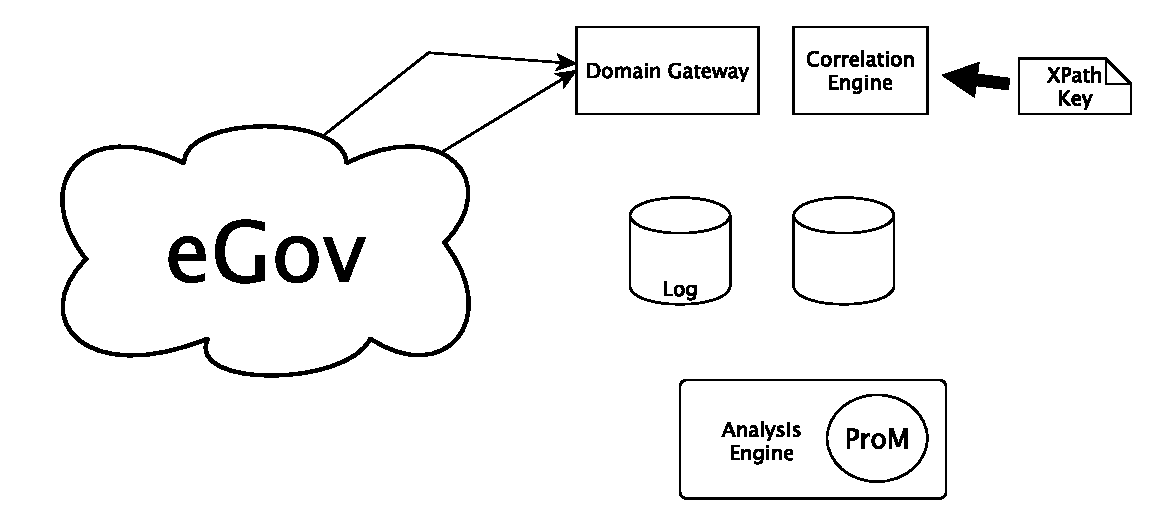
\includegraphics[scale=0.30]{./fig/Platform01}
%%   \end{center}

%% }

%% \frame{
%%   \begin{block}{Overall architecture}
    
%%     \begin{itemize}
%%     \item \alert{ProM} an existing process analysis framework
%%     \item \alert{OpenSPCoop} the most adopted  open source SPCoop implementation
%%     \end{itemize}

%%   \end{block}
  
%%   \begin{center}
%%     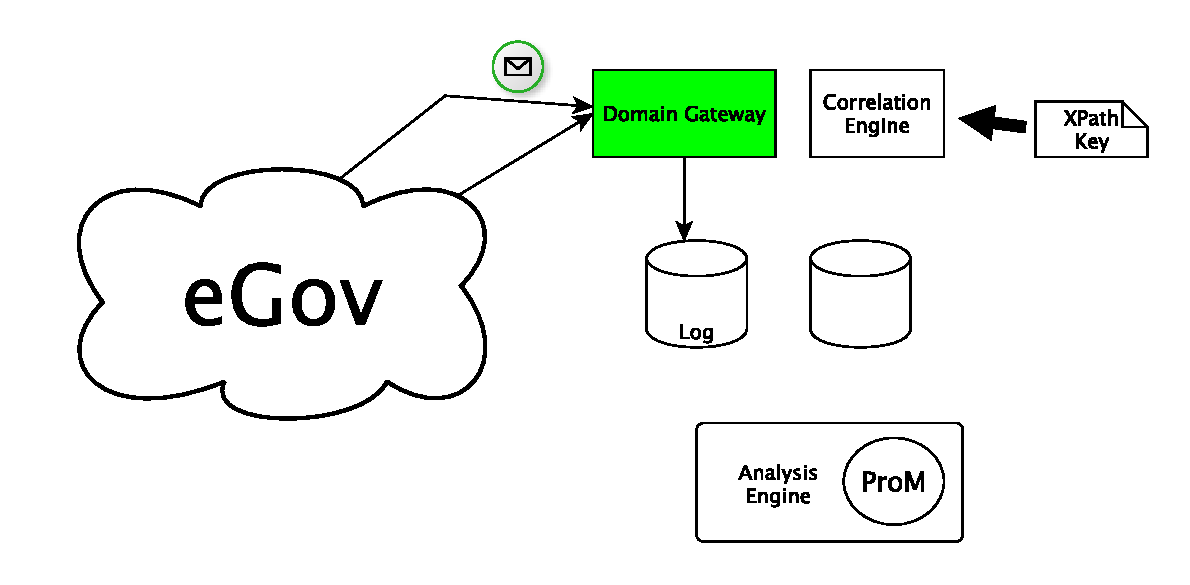
\includegraphics[scale=0.30]{./fig/Platform02}
%%   \end{center}

%%   \begin{itemize}
%%     \item eGov envelopes intercepted by Domain Gateway
%%     \item Domain Gateway stores message key information into the Log
%%       database
%%     %\item Domain Gateway performance are not affected by the analysis
%%     % \item <2-> Correlation engine groups SOAP request/response
%%     %   \begin{itemize}
%%     %     \item exploiting correlation sets (\alert{XPath})
%%     %     \item annotates process instances into log requests
%%     %     \item is externally triggered (e.g. cron/trigger)
%%     %   \end{itemize}
%%     % \item <3-> Analysis engine evaluates process metrics
%%     %   \begin{itemize}
%%     %     \item process definition stored in an external database (\alert{BPMN})
%%     %     \item process metrics stored into the log database
%%     %     \item is externally triggered (e.g. cron/trigger)
%%     %     \item fuffa su ProM
%%     %   \end{itemize}
%%   \end{itemize}
%% }

%% \frame{
%%   \begin{block}{Overall architecture}
    
%%     \begin{itemize}
%%     \item \alert{ProM} an existing process analysis framework
%%     \item \alert{OpenSPCoop} the most adopted  open source SPCoop implementation
%%     \end{itemize}

%%   \end{block}
  
%%   \begin{center}
%%     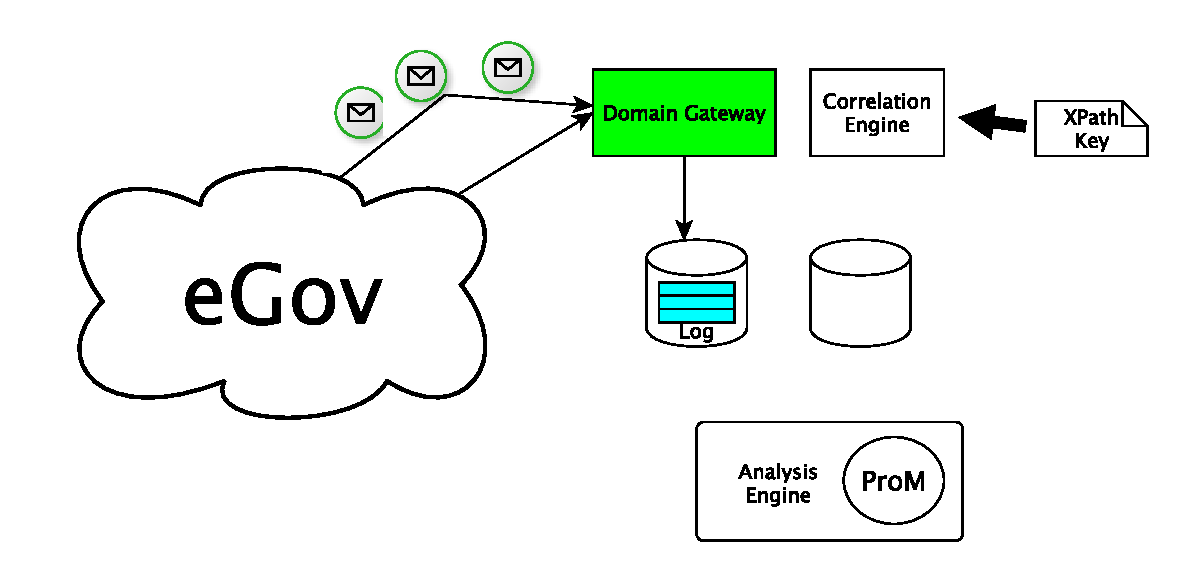
\includegraphics[scale=0.30]{./fig/Platform03}
%%   \end{center}

%%   \begin{itemize}
%%    \item eGov envelopes intercepted by Domain Gateway
%%     \item Domain Gateway stores message key information into the Log
%%       database
%%      \item Domain Gateway retrieves messages parts storing into the Log
%%       database
%%     %\item Domain Gateway performance are not affected by the analysis
%%     % \item <2-> Correlation engine groups SOAP request/response
%%     %   \begin{itemize}
%%     %     \item exploiting correlation sets (\alert{XPath})
%%     %     \item annotates process instances into log requests
%%     %     \item is externally triggered (e.g. cron/trigger)
%%     %   \end{itemize}
%%     % \item <3-> Analysis engine evaluates process metrics
%%     %   \begin{itemize}
%%     %     \item process definition stored in an external database (\alert{BPMN})
%%     %     \item process metrics stored into the log database
%%     %     \item is externally triggered (e.g. cron/trigger)
%%     %     \item fuffa su ProM
%%     %   \end{itemize}
%%   \end{itemize}
%% }

%% \frame{
%%   \begin{block}{Overall architecture}
    
%%     \begin{itemize}
%%     \item \alert{ProM} an existing process analysis framework
%%     \item \alert{OpenSPCoop} the most adopted  open source SPCoop implementation
%%     \end{itemize}

%%   \end{block}
  
%%   \begin{center}
%%     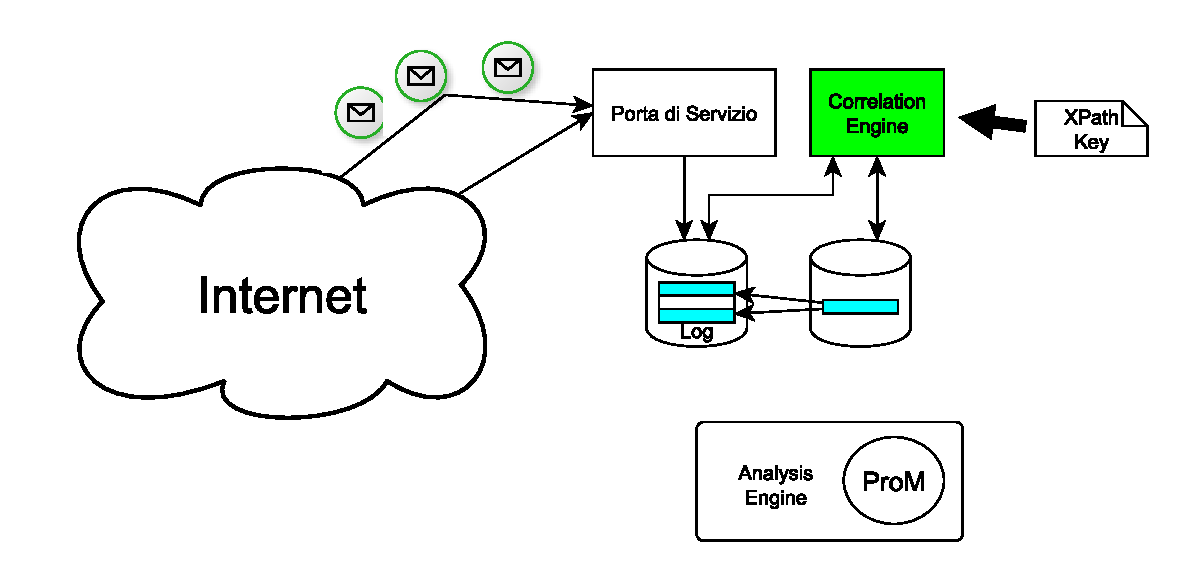
\includegraphics[scale=0.30]{./fig/Platform04}
%%   \end{center}

%%   \begin{itemize}
%%   \item eGov envelopes intercepted by Domain Gateway
%%     \item Domain Gateway stores message key information into the Log
%%       database
%%      \item Domain Gateway retrieves messages parts storing into the Log
%%       database
%%      \item Correlation engine groups SOAP request/response
%%        exploiting correlation sets (\alert{XPath})
%%      \item Service externally invoked (e.g. cron/trigger)
%%     % \item <3-> Analysis engine evaluates process metrics
%%     %   \begin{itemize}
%%     %     \item process definition stored in an external database (\alert{BPMN})
%%     %     \item process metrics stored into the log database
%%     %     \item is externally triggered (e.g. cron/trigger)
%%     %     \item fuffa su ProM
%%     %   \end{itemize}
%%   \end{itemize}
%% }

\begin{frame}{Architettura complessiva: integrazione di ProM in RUPOS}
  %% \begin{block}{}
    
  %%   \begin{itemize}
  %%   \item \alert{ProM} un framework per analisi di processi esistente
  %%   \item \alert{OpenSPCoop} the most adopted  open source SPCoop implementation
  %%   \end{itemize}

  %% \end{block}
  
  \begin{center}
    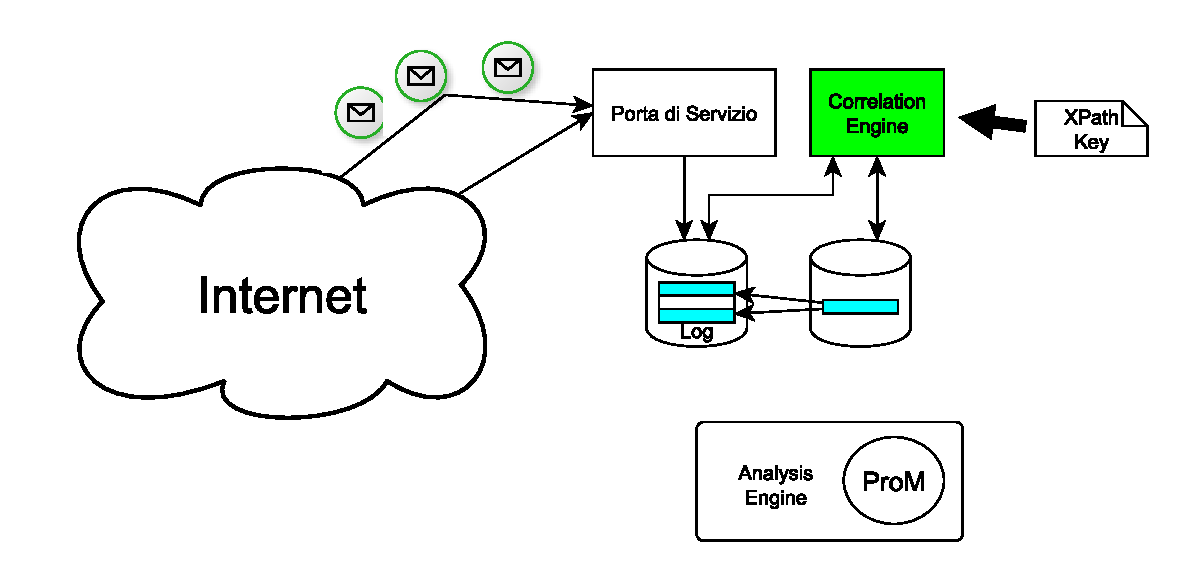
\includegraphics[scale=0.30]{./fig/Platform04}
  \end{center}

  \begin{itemize}
  \item I messaggi SOAP tra attori del processo vengono intercettati dalla Porta di Servizio (PdS)
    \item La PdS memorizza informazioni essenziali dei messaggi nel log
     \item La PdS estrae parti dei messaggi memorizzandoli nel database dei log
     \item Il Motore di Correlazione raggruppa i messaggi in istanze di processi usando ``correlation sets'' (\alert{XPath})
%     \item Service externally invoked (e.g. cron/trigger)
    \item I log di istanze di processi vengono trasformati in tracce di eventi corrispondenti a transizioni della Rete di Petri
%%  Gli eventi del log 

%% l framework di analisi calcola le metriche e annota il modello BPMN con i risultati
%    \item Service externally invoked (e.g. cron/trigger)
%    \item implements a context to integrate ProM into JBoss AS
  \end{itemize}
\end{frame}

%%% Local Variables: 
%%% mode: latex
%%% TeX-master: "main"
%%% End: 
